\documentclass[t,12pt]{beamer}

%liste des packages utilsé
\usepackage[T1]{fontenc}
\usepackage[french]{babel}
\usepackage[utf8]{inputenc}
\usepackage{graphicx}
\usepackage{pslatex}
%definition d'une couleur pour les titres
\definecolor{grisbleu}{rgb}{0,0,153}


%definition du thème
\useoutertheme[height=0pt,left]{sidebar}
\usecolortheme{seahorse}
\setbeamercolor*{titlelike}{parent=structure}
\useinnertheme{circles}
\setbeamertemplate{frametitle}[default][right]


% contenu de la page de titre
\title{Projet tuteuré}
\subtitle{\tiny{UFWI}}
\author{BAROTTE Simon, FROLICH Valentin, PIERRÉ Cyril, ROBIN Maxime}

\begin{document}

%------- page de titre --------
\frame{\titlepage}

% --------- Sommaire ---------

\begin{frame} 
	\begin{center}{\Large Somaire }\end{center}
	\tableofcontents[currentsection]       %genere un somaire automatique (avec les \section)
\end{frame} 

%-----page Objectif-----------
\section{Introduction}                                                    %utilisé pour la generation du sommaire
\begin{frame}                                                         %définit le debut de la page
    \begin{center}{\textcolor{grisbleu}{\Large Introduction}}\end{center} %centre et colore le titre
    \begin{itemize}                                                   %definie une liste
	\item Intro
	\item Algo
\end{itemize}
\end{frame}                                                            %définit la fin de la page

\section{Modules}                                                    %utilisé pour la generation du sommaire
\begin{frame}                                                         %définit le debut de la page
    \begin{center}{\textcolor{grisbleu}{\Large Modules}}\end{center} %centre et colore le titre
    \begin{itemize}                                                   %definie une liste
	\item Authentification
	\newline
	\item Filtred
	\newline
	\item Rcpd
	\newline
	\item Client
\end{itemize}
\end{frame}                                                           %définit la fin de la page

	  \subsection{Authentification}
	  \begin{frame}                                                         %définit le debut de la page
	      \begin{center}{\textcolor{grisbleu}{\Large Authentification}}\end{center} %centre et colore le titre
	      \begin{itemize}                                                 %definie une liste
		\item Introduction
		\newline
		\item Configuration
		 \newline
		\item Fonctionnement de l'authentification
	  \end{itemize}
	  \end{frame} 


	  \begin{frame}                                                         %définit le debut de la page
	      \begin{center}{\textcolor{grisbleu}{\Large Authentification}}\end{center} %centre et colore le titre
		  \begin{center}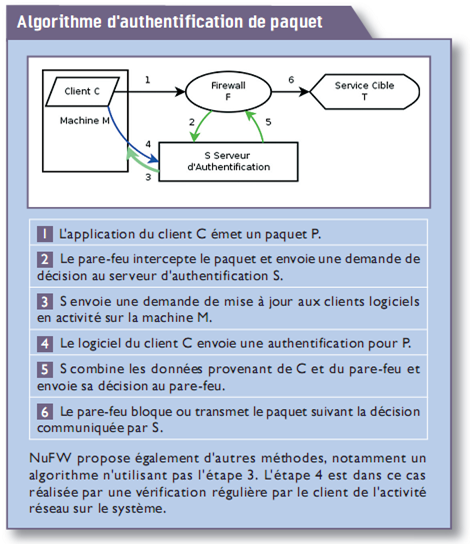
\includegraphics[width=5cm,height=6cm]{images/auth.png}\end{center}
	  \end{frame} 

	  \subsection{Filtred}
	  \begin{frame}                                                         %définit le debut de la page
	      \begin{center}{\textcolor{grisbleu}{\Large Filtred}}\end{center} %centre et colore le titre
	      \begin{itemize}                                                   %definie une liste
		\item Introduction
		\newline
		\item Fonctionnalités
		\newline
		\item Fichier de configuration
	  \end{itemize}
	  \end{frame} 

	  \subsection{Rcpd}
	  \begin{frame}                                                         %définit le debut de la page
	      \begin{center}{\textcolor{grisbleu}{\Large Rcpd}}\end{center} %centre et colore le titre
	      \begin{itemize}                                                   %definie une liste
		\item
	  \end{itemize}
	  \end{frame} 

	  \subsection{Client}
	  \begin{frame}                                                         %définit le debut de la page
	      \begin{center}{\textcolor{grisbleu}{\Large Client}}\end{center} %centre et colore le titre
	      \begin{itemize}                                                   %definie une liste
		\item Introduction
		\newline
		\item Différent client disponnible
		\newline
		\item Multi-plateformes
		\newline
		\begin{center}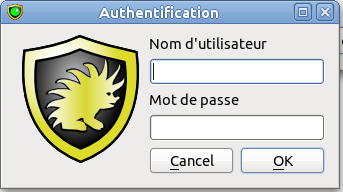
\includegraphics[width=4cm,height=3cm]{images/nuapp.png}\end{center}
	  \end{itemize}
	  \end{frame} 

\section{Comparaison}                                                    %utilisé pour la generation du sommaire
\begin{frame}                                                         %définit le debut de la page
    \begin{center}{\textcolor{grisbleu}{\Large Comparaison}}\end{center} %centre et colore le titre
    \begin{itemize}                                                   %definie une liste
	\item Différentes solution de pare feu
\begin{center}AuthPF, NUFW, Cyberoam, CheckPoint\end{center}
	\item Installation, mise en oeuvre
	\item Modularité
        \item Sécutité
        \item Intéret
\end{itemize}
\end{frame}                                                            %définit la fin de la page


\section{Problèmes et Conclusion}                                                    %utilisé pour la generation du sommaire
\begin{frame}                                                         %définit le debut de la page
    \begin{center}{\textcolor{grisbleu}{\Large Problèmes et Conclusion}}\end{center} %centre et colore le titre
    \begin{itemize}                                                   %definie une liste
	\item Problèmes lors de l'installation
	\item Problèmes de configuration
	\item Conclusion
\end{itemize}
\end{frame}                                                            %définit la fin de la page
	\subsection{Problèmes lors de l'installation}
		\begin{frame}                                                         %définit le debut de la page
    \begin{center}{\textcolor{grisbleu}{\Large Problèmes lors de l'installation}}\end{center} %centre et colore le titre
		\begin{itemize}
			\item Problèmes de dépendances
			\newline
			\item Problèmes d'obsolèscence
			\newline		
			\item Problème dans le code
			\newline
			\item Peu de documentation
		\end{itemize}
		\end{frame}

	\subsection{Problèmes de configuration}
		\begin{frame}                                                         %définit le debut de la page
    \begin{center}{\textcolor{grisbleu}{\Large Problèmes de configuration}}\end{center} %centre et colore le titre
		\begin{itemize}
			\item Problèmes de librairies
			\newline
			\newline
			\item Problèmes de certificats
		\end{itemize}
		\end{frame}


	\subsection{Conclusion}
		\begin{frame}                                                         %définit le debut de la page
    \begin{center}{\textcolor{grisbleu}{\Large Conclusion}}\end{center} %centre et colore le titre
		\begin{itemize}
			\item Projet Libre
			\newline
			\item Projet ayant sa place dans la sécurité des entreprises
			\newline
			\item Logiciels modulables et multi-plateformes
			\newline
			\item Des lacunes 
		\end{itemize}
		\end{frame}


\end {document}
